\documentclass[12pt]{article}
\usepackage{times}
\usepackage[letterpaper, margin=1in]{geometry}
\usepackage{pdfpages}
\usepackage{graphicx}
\usepackage{float}
\usepackage{fancyhdr}
\usepackage{lscape}
\usepackage{indentfirst}
\usepackage{cleveref}
\usepackage{enumitem}
\fancyhf{}
\newcommand{\ph}{\framebox[48pt]{\rule{0pt}{12pt}}}
\begin{document}
% Title Page
{\noindent\LARGE\fontfamily{phv}\selectfont High Altitude Class 3 Filing}\newline
{\noindent\Large\fontfamily{phv}\selectfont Mines Rocket Club}\newline

Document prepared by Tom Powell, with information furnished by:
\begin{itemize}
    \item Will Swegles,
    \item Ashle Jantzen,
    \item Caleb Mark,
    \item Andrew Wu
\end{itemize}
\clearpage
% FAA Form 7711
% To Update: Edit the PDF "media/Form7711.pdf" and print the PDF 
% to the file "media/FilledForm7711.pdf" and recompile.
\pagestyle{empty}
\includepdf[pages={2,3}]{media/FilledForm7711.pdf}
\clearpage 
% USGS 7.5 minute topographic quandrangle per directions on 7711.
\pagestyle{empty}
\begin{landscape}
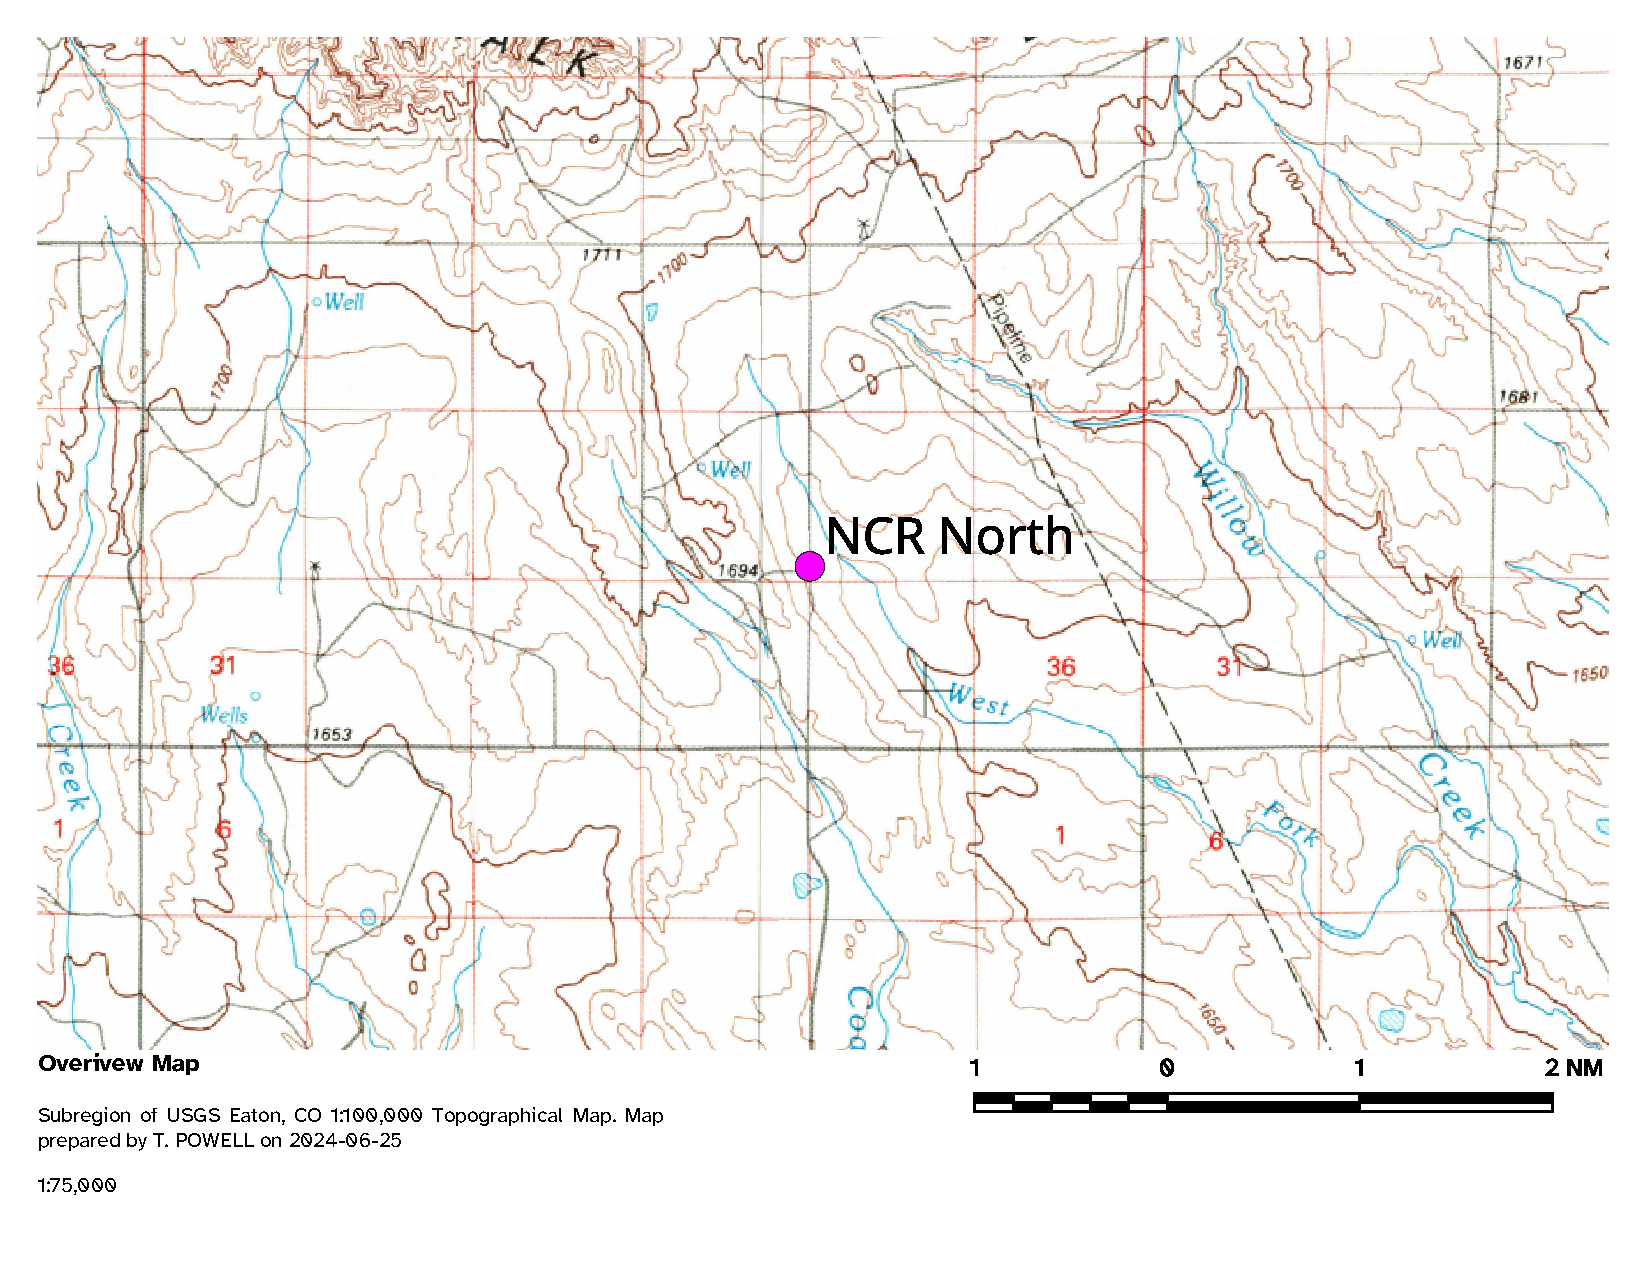
\includepdf[pages=-]{media/primary-ncrnorth.pdf}
\end{landscape}
\clearpage
\pagestyle{fancy}
\noindent{\Large\fontfamily{phv}\selectfont Supplemental Information for Item 5, FAA Form 7711-2}\newline
\section{Description of Systems}
\subsection{Lower Stage (Booster)}
\subsubsection{Propulsion}
\begin{enumerate}[label=(\alph*)]
    \item Ammonium Perchlorate Composite Propellant (APCP); 80\% solids, 10\% Aluminum.
    \item \ph inches of characterized propellant in \ph diameter \ph type grains; phenolic liner, epoxy bonded grains, assembled per OEM instructions.
    \item Characteristics
    \begin{table}[H]
        % Get this data from running burnsim over an existing motor file.
        \centering
        \caption{Motor Characteristics, generated with BurnSim version \ph.}
        \begin{tabular}{|l|l|l|}
            \hline
            Kn: \ph & Max Pc \ph & Volumetric Loading: \ph \\ \hline
            Web: \ph & Burn Time \ph & Propellant Length: \ph \\ \hline
            Mass: \ph & Motor Class \ph & Delivered Isp: \ph \\ \hline
        \end{tabular}
    \end{table}
    \item Motor is \ph long, \ph diameter, \ph wall drawn over mandrel (DOM) tubing,
    OEM supplied composite nozzle with steel retention cap.
    The motor is retained into the airframe using head end motor retention,
    no loading from recovery systems is placed on the retainer-motor interface.
\end{enumerate}
\subsubsection{Airframe}
\begin{enumerate}[label=(\alph*)]
    \item Nominal outer body tube diameter of \ph in, length of \ph in.
    \item Internal motor retention bulkhead FDM printed from polycarbonate.
    \item Fins constructed from milled \& routed \ph plate.
    \item Fillets made with Smooth-On MT-13 pre-thickened epoxy.
    \item Fin can receives \ph layers of \ph layup, with alternating weave directions.
\end{enumerate}
\subsubsection{Avionics}
\begin{enumerate}[label=(\alph*)]
    \item Motor is ignited by ground launch control box.
    \item Altus Metrum TeleMetrum (GPS, Barometric, Accelerometer)
    \begin{enumerate}[label=(\arabic*)]
        \item Drives stage separation charge.
        \item Drives lower stage recovery deployment charge.
    \end{enumerate}
    \item Jolly Logic Chute Release
    \begin{enumerate}[label=(\arabic*)]
        \item Ejected by recovery deployment charge with both drogue and main parachutes.
        \item Releases main parachute at \ph feet AGL.
    \end{enumerate}
\end{enumerate}
\subsubsection{Recovery}
\begin{enumerate}[label=(\alph*)]
    \item \ph inch drogue parachute. \ph feet per second descent rate.
    \item \ph inch main parachute. \ph feet per second descent rate.
\end{enumerate}
\subsection{Upper Stage (Sustainer)}
\subsubsection{Propulsion}
\begin{enumerate}[label=(\alph*)]
    \item Ammonium Perchlorate Composite Propellant (APCP); 80\% solids, 10\% Aluminum.
    \item \ph inches of characterized propellant in \ph diameter \ph type grains; phenolic liner, epoxy bonded grains, assembled per OEM instructions.
    \item Characteristics
    \begin{table}[H]
        % Get this data from running burnsim over an existing motor file.
        \centering
        \caption{Motor Characteristics, generated with BurnSim version \ph.}
        \begin{tabular}{|l|l|l|}
            \hline
            Kn: \ph & Max Pc \ph & Volumetric Loading: \ph \\ \hline
            Web: \ph & Burn Time \ph & Propellant Length: \ph \\ \hline
            Mass: \ph & Motor Class \ph & Delivered Isp: \ph \\ \hline
        \end{tabular}
    \end{table}
    \item Motor is \ph long, \ph diameter, \ph wall drawn over mandrel (DOM) tubing,
    OEM supplied composite nozzle with steel retention cap.
    The motor is retained into the airframe using head end motor retention,
    no loading from recovery systems is placed on the retainer-motor interface.
\end{enumerate}
\subsubsection{Airframe}
\begin{enumerate}[label=(\alph*)]
    \item Nominal outer body tube diameter of \ph in, length of \ph in.
    \item Internal motor retention bulkhead FDM printed from polycarbonate.
    \item Fins constructed from milled \& routed \ph plate.
    \item Fillets made with Smooth-On MT-13 pre-thickened epoxy.
    \item Fin can receives \ph layers of \ph layup, with alternating weave directions.
\end{enumerate}
\subsubsection{Avionics}
\begin{enumerate}[label=(\alph*)]
    \item Motor is ignited by ground launch control box.
    \item Altus Metrum TeleMetrum (GPS, Barometric, Accelerometer)
    \begin{enumerate}[label=(\arabic*)]
        \item Drives stage separation charge.
        \item Drives lower stage recovery deployment charge.
    \end{enumerate}
    \item Jolly Logic Chute Release
    \begin{enumerate}[label=(\arabic*)]
        \item Ejected by recovery deployment charge with both drogue and main parachutes.
        \item Releases main parachute at \ph feet AGL.
    \end{enumerate}
\end{enumerate}
\subsubsection{Recovery}
\begin{enumerate}[label=(\alph*)]
    \item \ph inch drogue parachute. \ph feet per second descent rate.
    \item \ph inch main parachute. \ph feet per second descent rate.
\end{enumerate}
\section{Operational Properties}
\subsection{Site Properties}
\begin{table}[H]
    \centering
    \caption{Launch Site Parameters}
    \begin{tabular}{|l|l|}
        \hline
        Tower Height & \ph in \\ \hline
        Launch Site Altitude & 5462.6 ft MSL \\ \hline
        Estimated Landing Site Altitude & 5400 ft MSL \\ \hline
        Site Longitude & 104$^\circ$ 38.322' W \\ \hline
        Site Latitude & 40$^\circ$ 53.134' N \\ \hline
        Typical Site Temperature & \ph \\ \hline
        Typical Site Pressure & \ph \\ \hline
    \end{tabular}
\end{table}
\subsection{Maximum Altitude and Maximum Range}
\subsubsection{Methods}
Highest altitude and maximum range simulations were attained using RASAero version \ph aerodynamic performance data.
Wind data was collated from observations recorded at the Eaton, CO\footnote{EATON 4.3 ENE, CO US} weather station.
Resultant collated data was provided to RS-Pro version\ph.
\begin{table}[H]
    \centering
    \caption{Maximum altitude and range.}
    \label{tab:winds}
    \begin{tabular}{|p{1in}|p{1in}|p{1in}|p{1in}|p{1in}|p{1in}|}
        \hline
        Wind State & Launch Orientation & Booster Altitude & Sustainer Altitude & Booster Range & Sustainer Range \\ \hline
        No Wind    & \ph                & \ph              & \ph                & \ph           &  \ph \\ \hline
        Typ. 08:00 Winds    & \ph                & \ph              & \ph                & \ph           & \ph \\ \hline
        Typ. 12:00 Winds    & \ph                & \ph              & \ph                & \ph           & \ph \\ \hline
        Typ. 16:00 Winds    & \ph                & \ph              & \ph                & \ph           & \ph \\ \hline
    \end{tabular}
\end{table}
\subsection{Static Stability Characteristics}
\begin{table}[H]
    \centering
    \begin{tabular}{|l|l|l|}
        \hline
        Mach Number & C.P. (in) & Stability/Static Margin (calibers) \\ \hline
        0.10        & \ph       &  \ph \\ \hline
        1.0         & \ph       & \ph \\ \hline
        2.0         & \ph       & \ph \\ \hline
        \ph (Max + 5\%)         & \ph       & \ph \\ \hline
    \end{tabular}
\end{table}
% Refer to the example document for what to include in these plots.
\subsection{Dynamic Stability Characteristics}
\begin{figure}
    \centering
    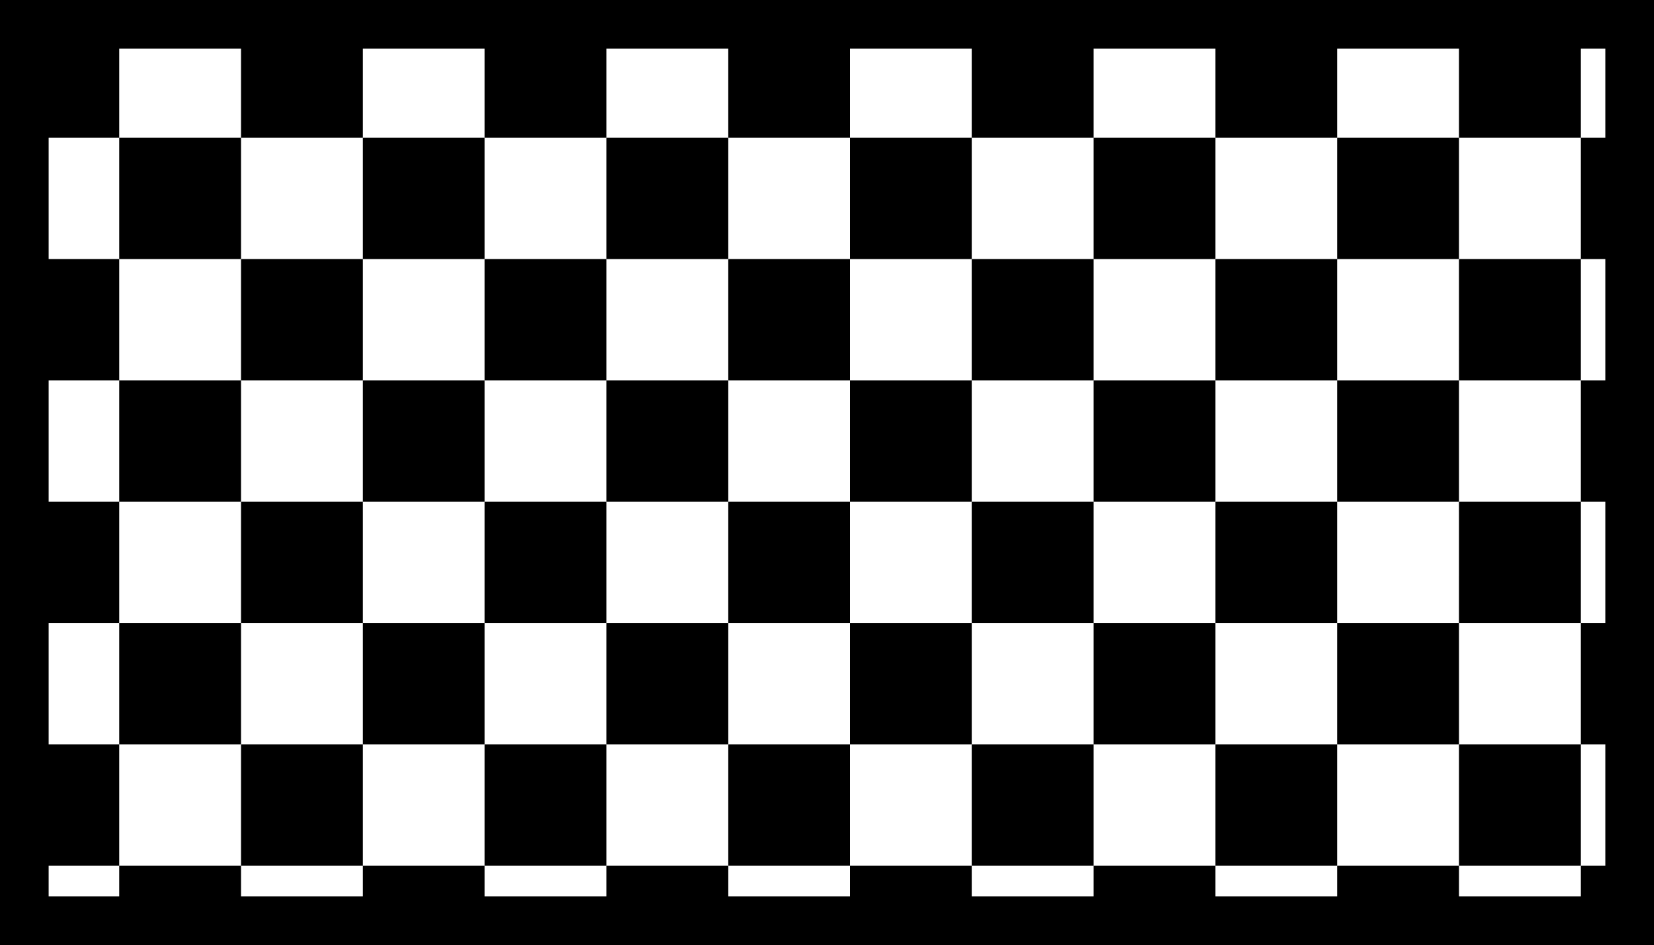
\includegraphics[width=.8\textwidth]{media/dynstab.png}
    \caption{Dynamic stability properties of the system.}
\end{figure}
\subsection{Mass \& Thrust Characteristics}
\begin{figure}
    \centering
    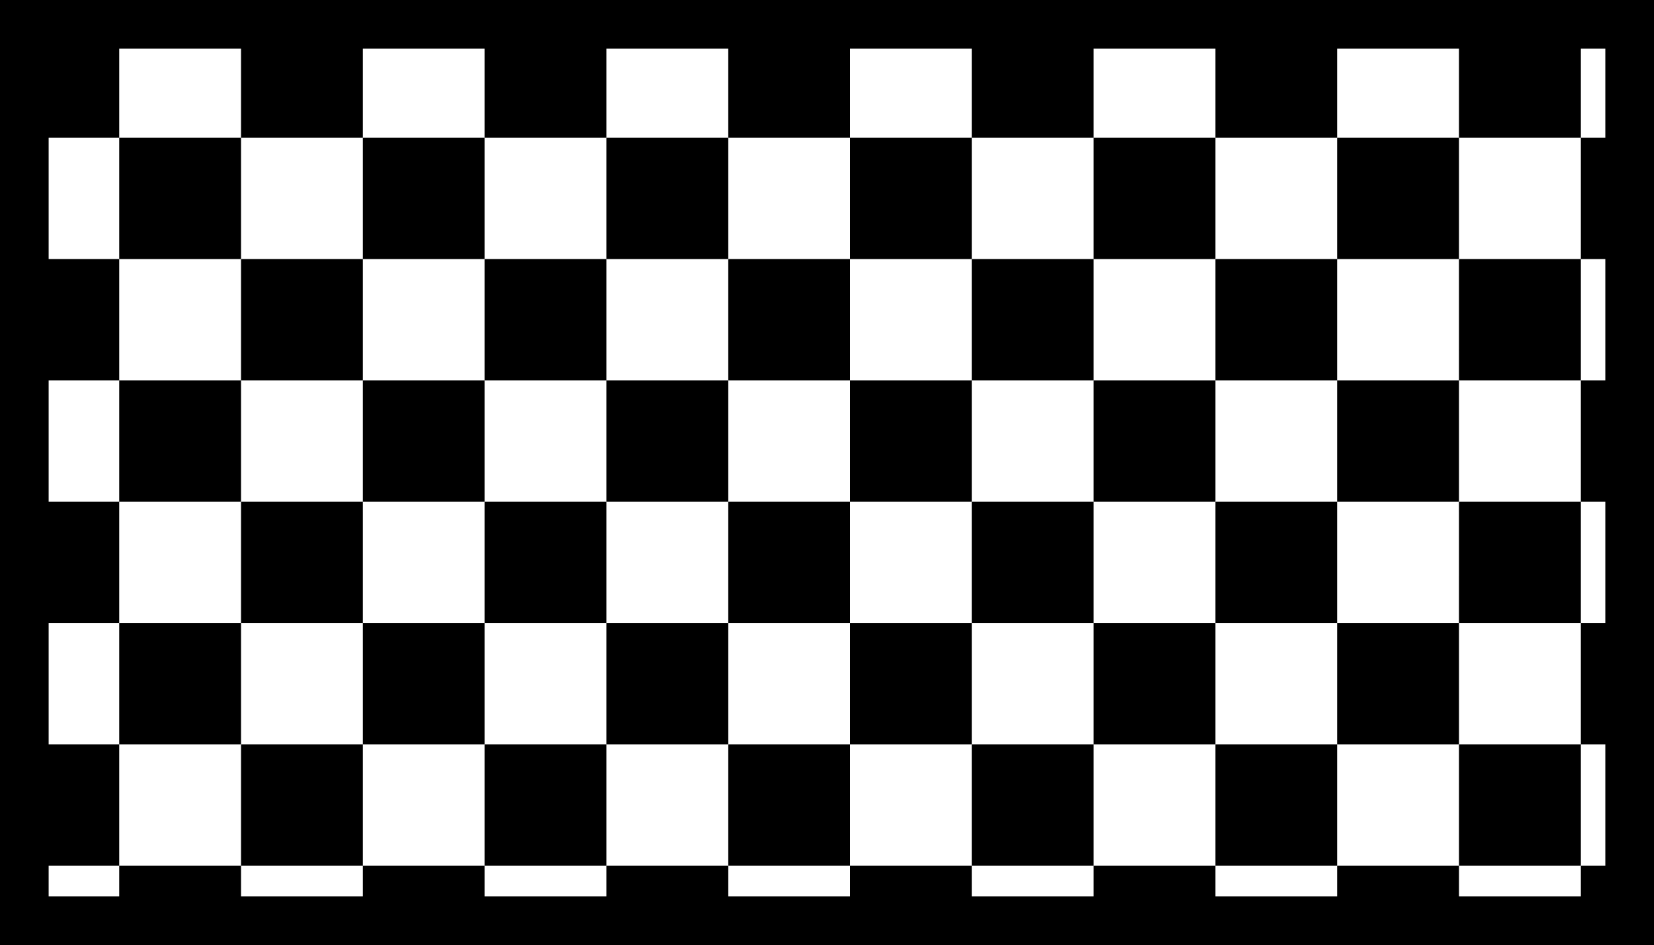
\includegraphics[width=.8\textwidth]{media/massthrust.png}
    \caption{Mass and thrust properties of the system.}
\end{figure}
\subsection{$C_p$, $C_n$, and Drag Characteristics}
\begin{figure}
    \centering
    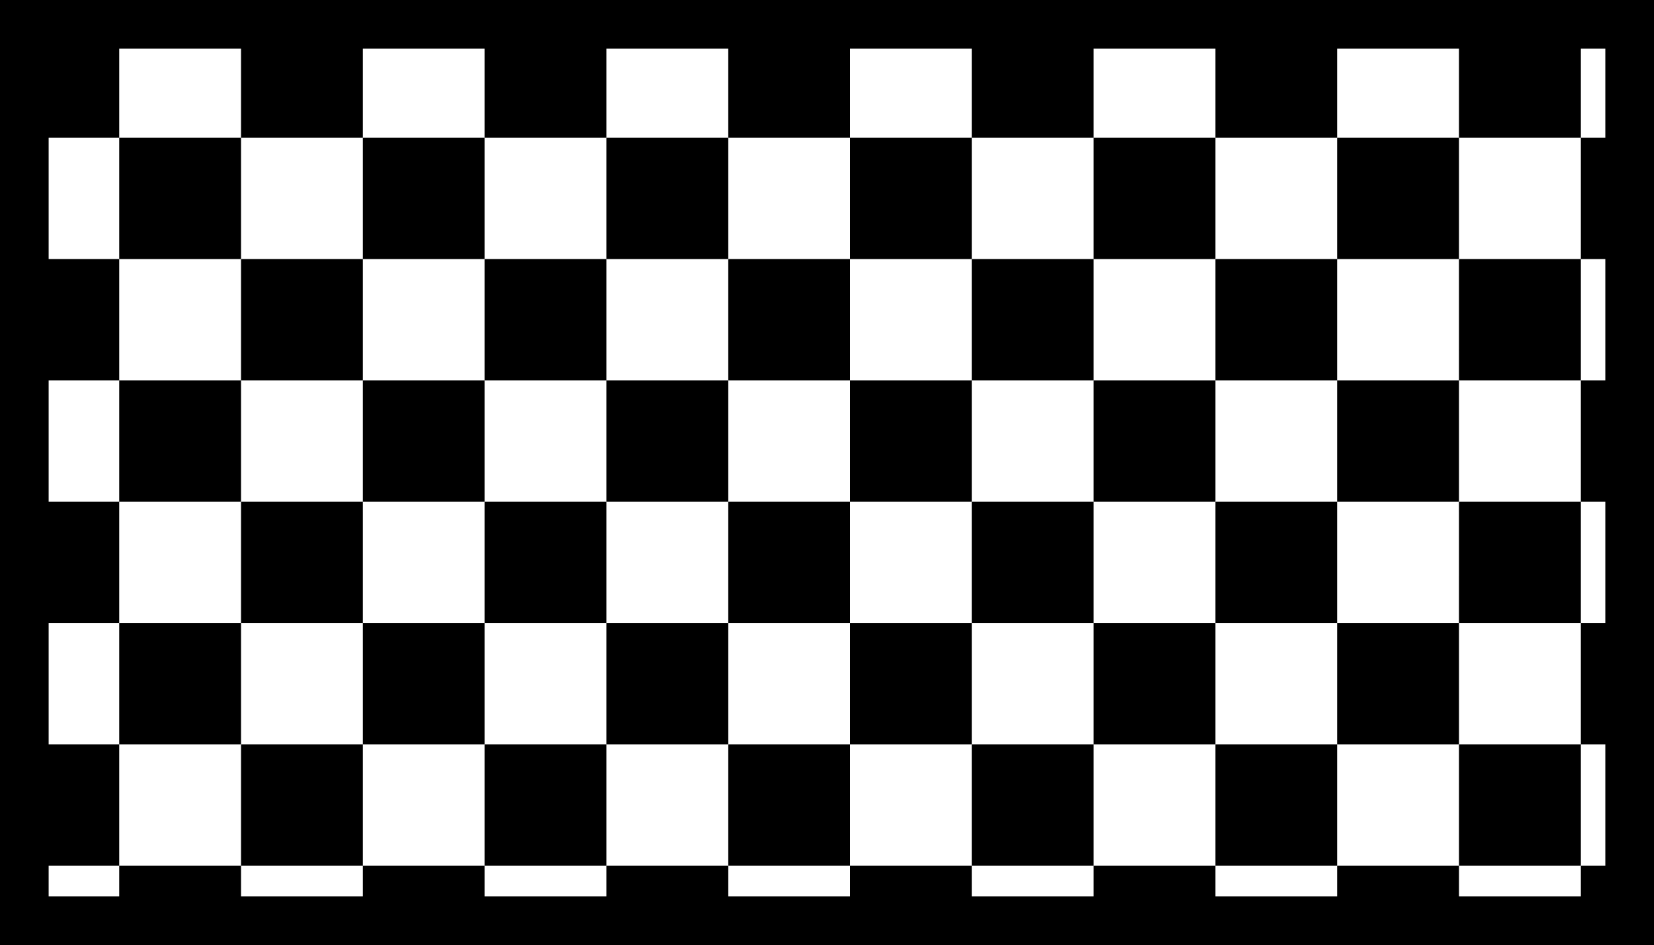
\includegraphics[width=.8\textwidth]{media/aero1.png}
    \caption{Aerodynamic properties of the system.}
\end{figure}
\subsection{$C_p$, $C_g$, and Mass Characteristics}
\begin{figure}
    \centering
    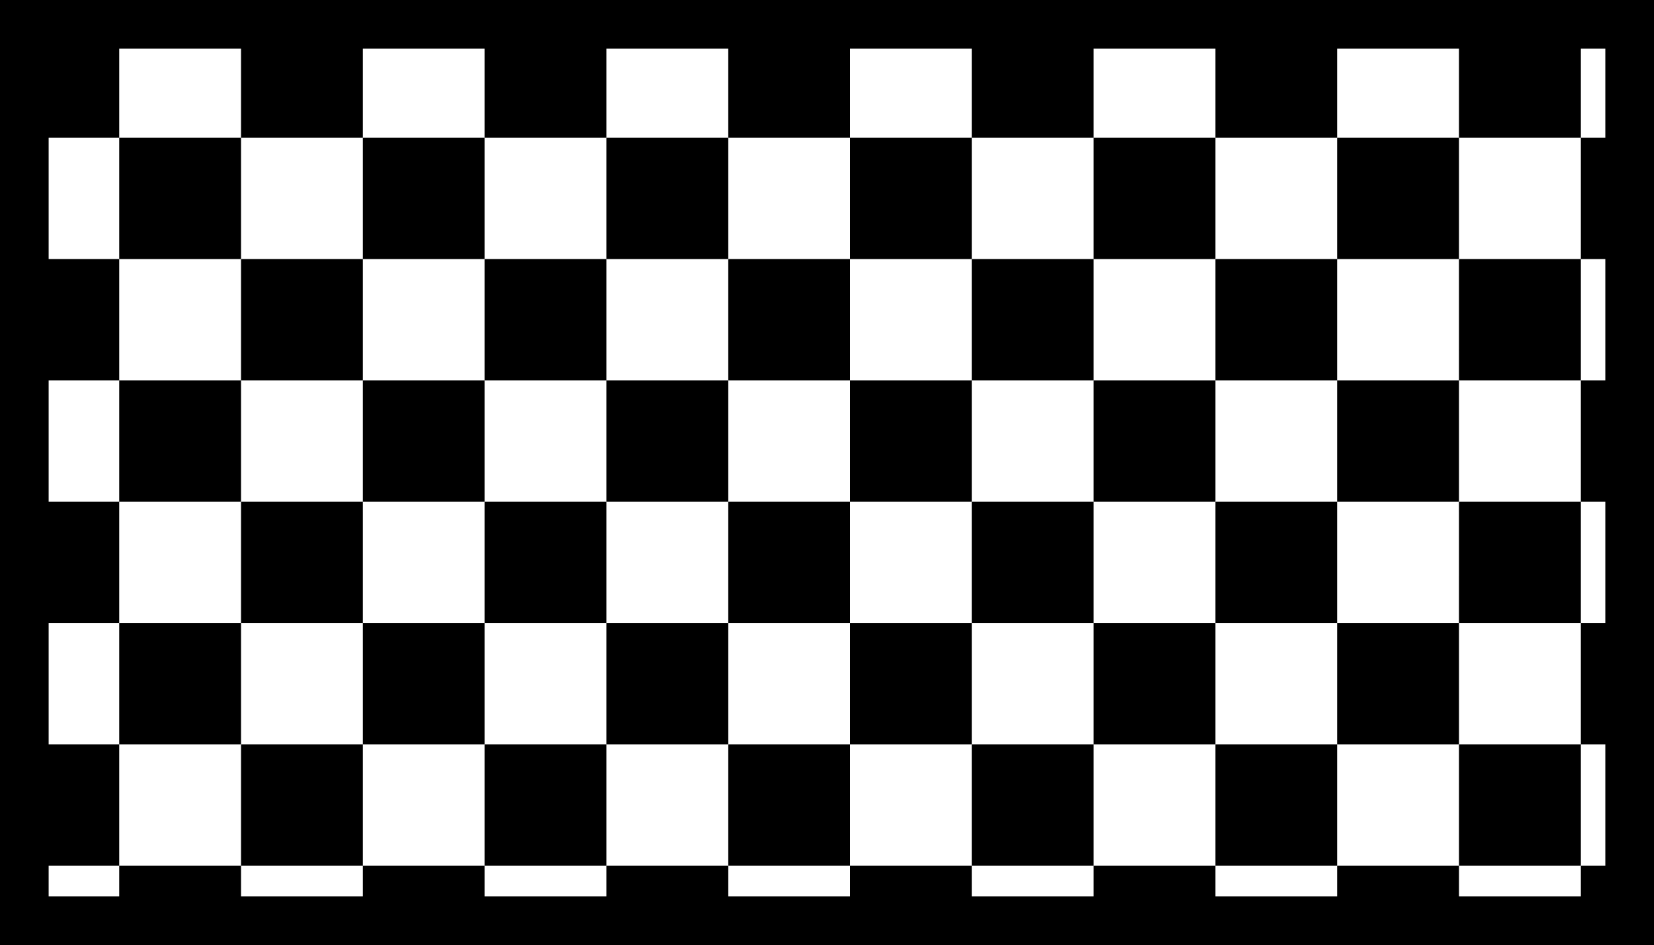
\includegraphics[width=.8\textwidth]{media/aero2.png}
    \caption{Continued aerodynamic properties of the system.}
\end{figure}
\subsection{Recovery Dispersion Characteristics}
For each of the wind states defined in \cref{tab:winds},
recovery dispersion calculations were run.
\subsubsection{No Wind}
\begin{figure}
    \centering
    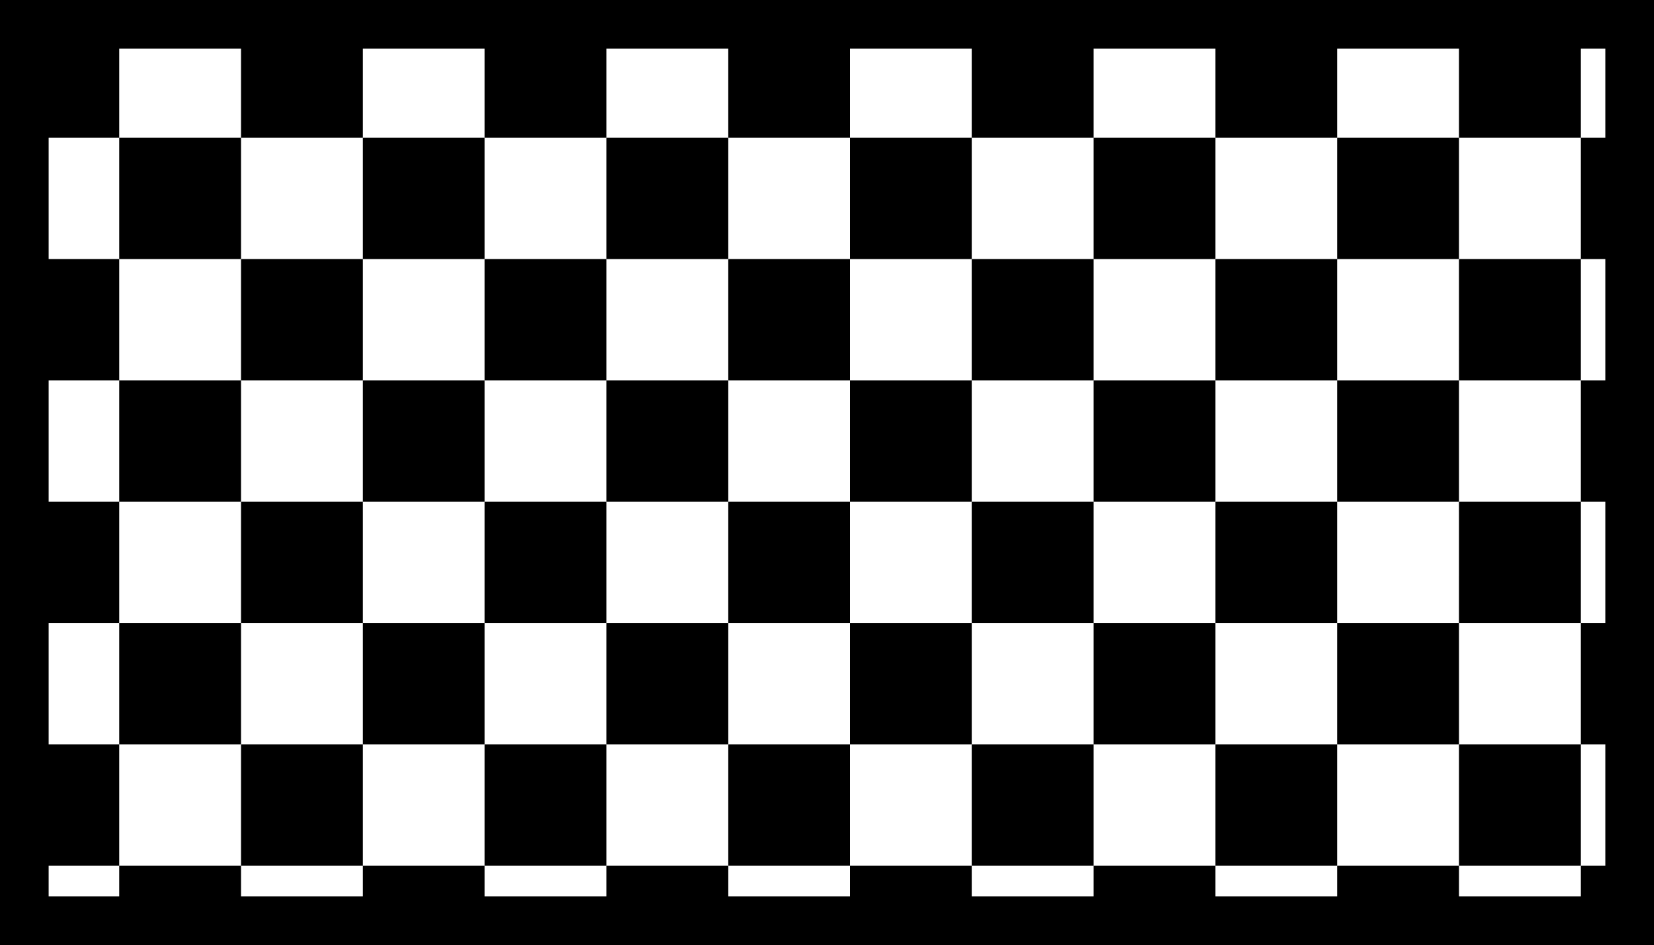
\includegraphics[width=.8\textwidth]{media/nowind.png}
    \caption{Recovery dispersion with no wind.}
\end{figure}
\subsubsection{Typ. 08:00 Winds}
\begin{figure}
    \centering
    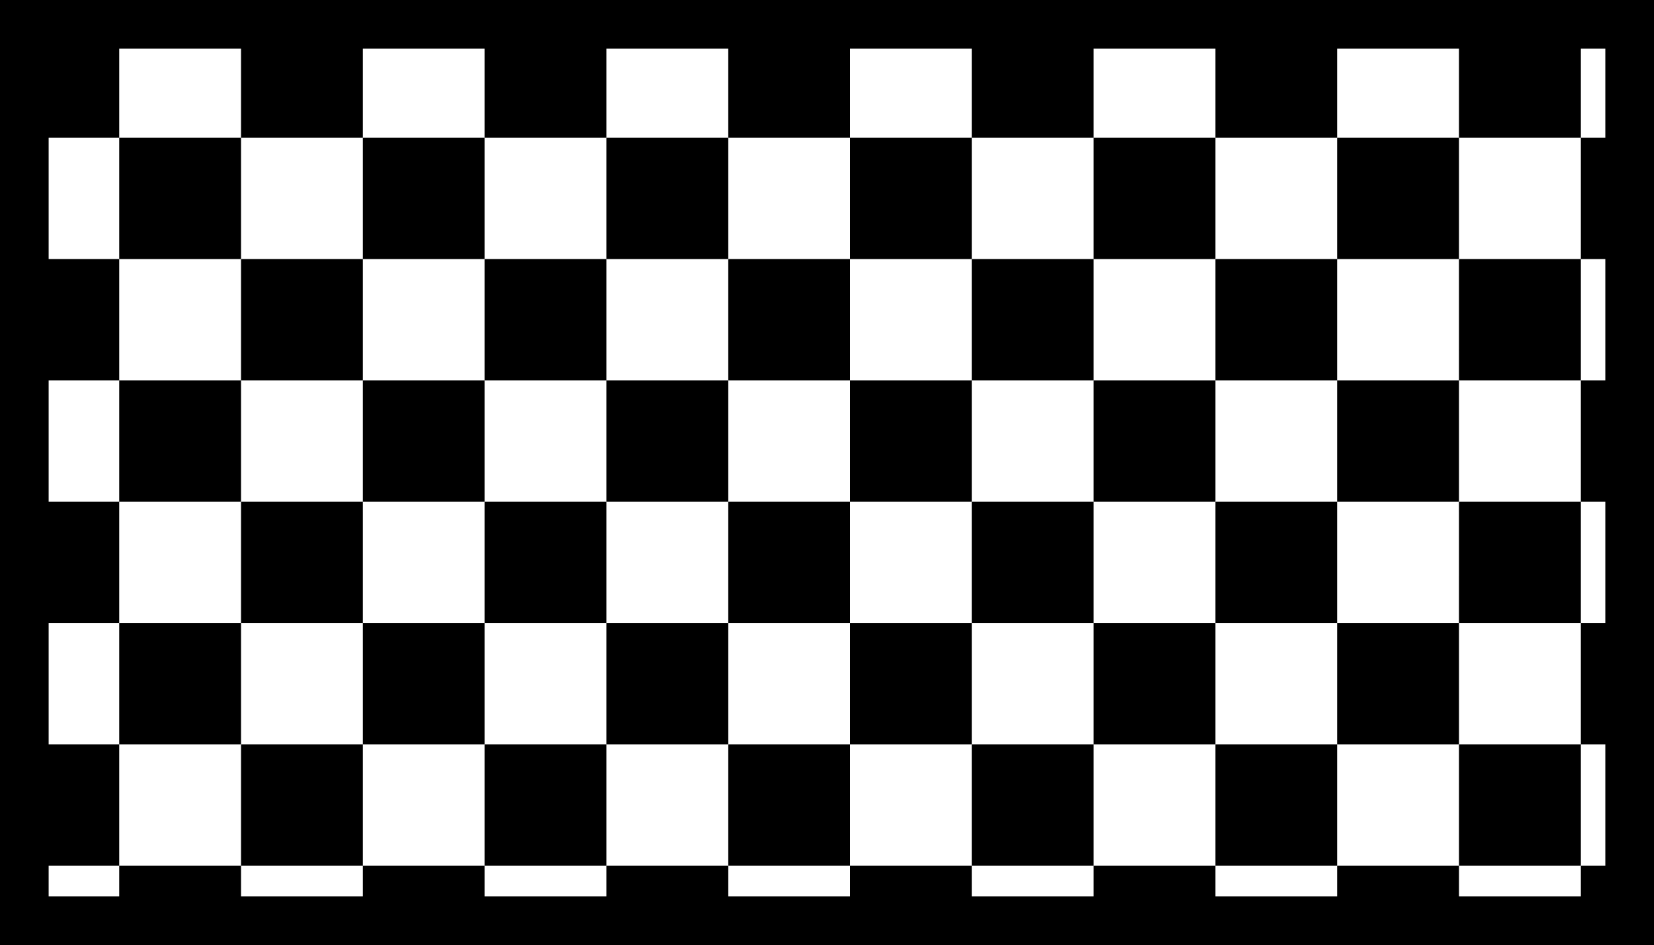
\includegraphics[width=.8\textwidth]{media/0800wind.png}
    \caption{Recovery dispersion with wind typical to 08:00 on the site.}
\end{figure}
\subsubsection{Typ. 12:00 Winds}
\begin{figure}
    \centering
    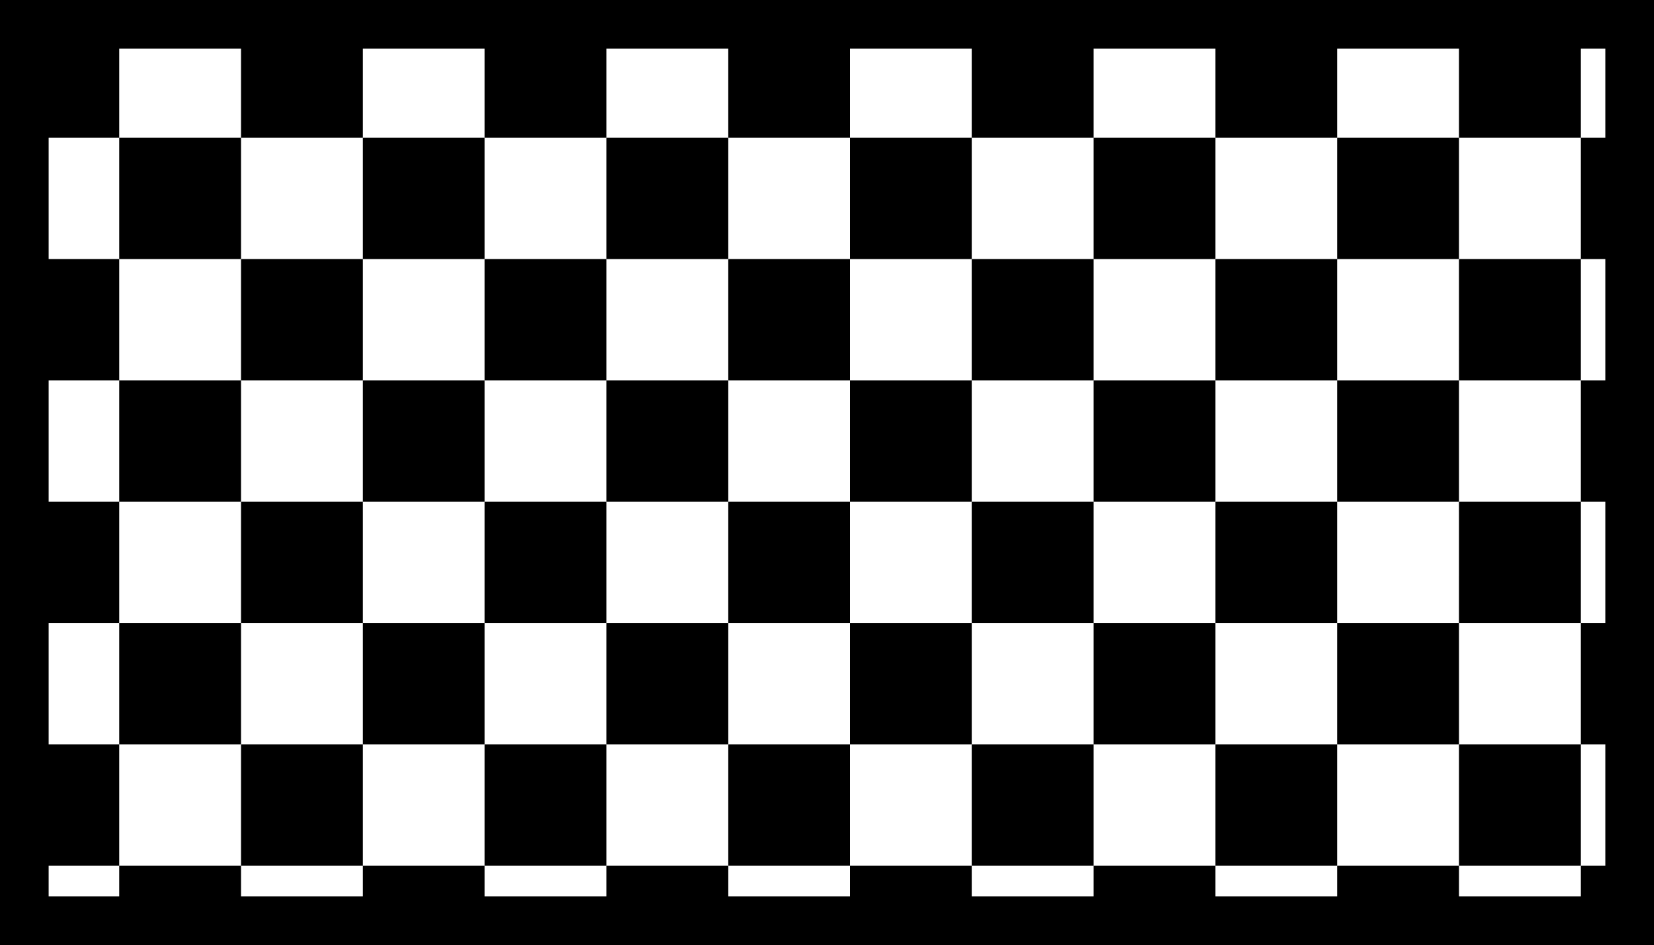
\includegraphics[width=.8\textwidth]{media/1200wind.png}
    \caption{Recovery dispersion with wind typical to 12:00 on the site.}
\end{figure}
\subsubsection{Typ. 16:00 Winds}
\begin{figure}
    \centering
    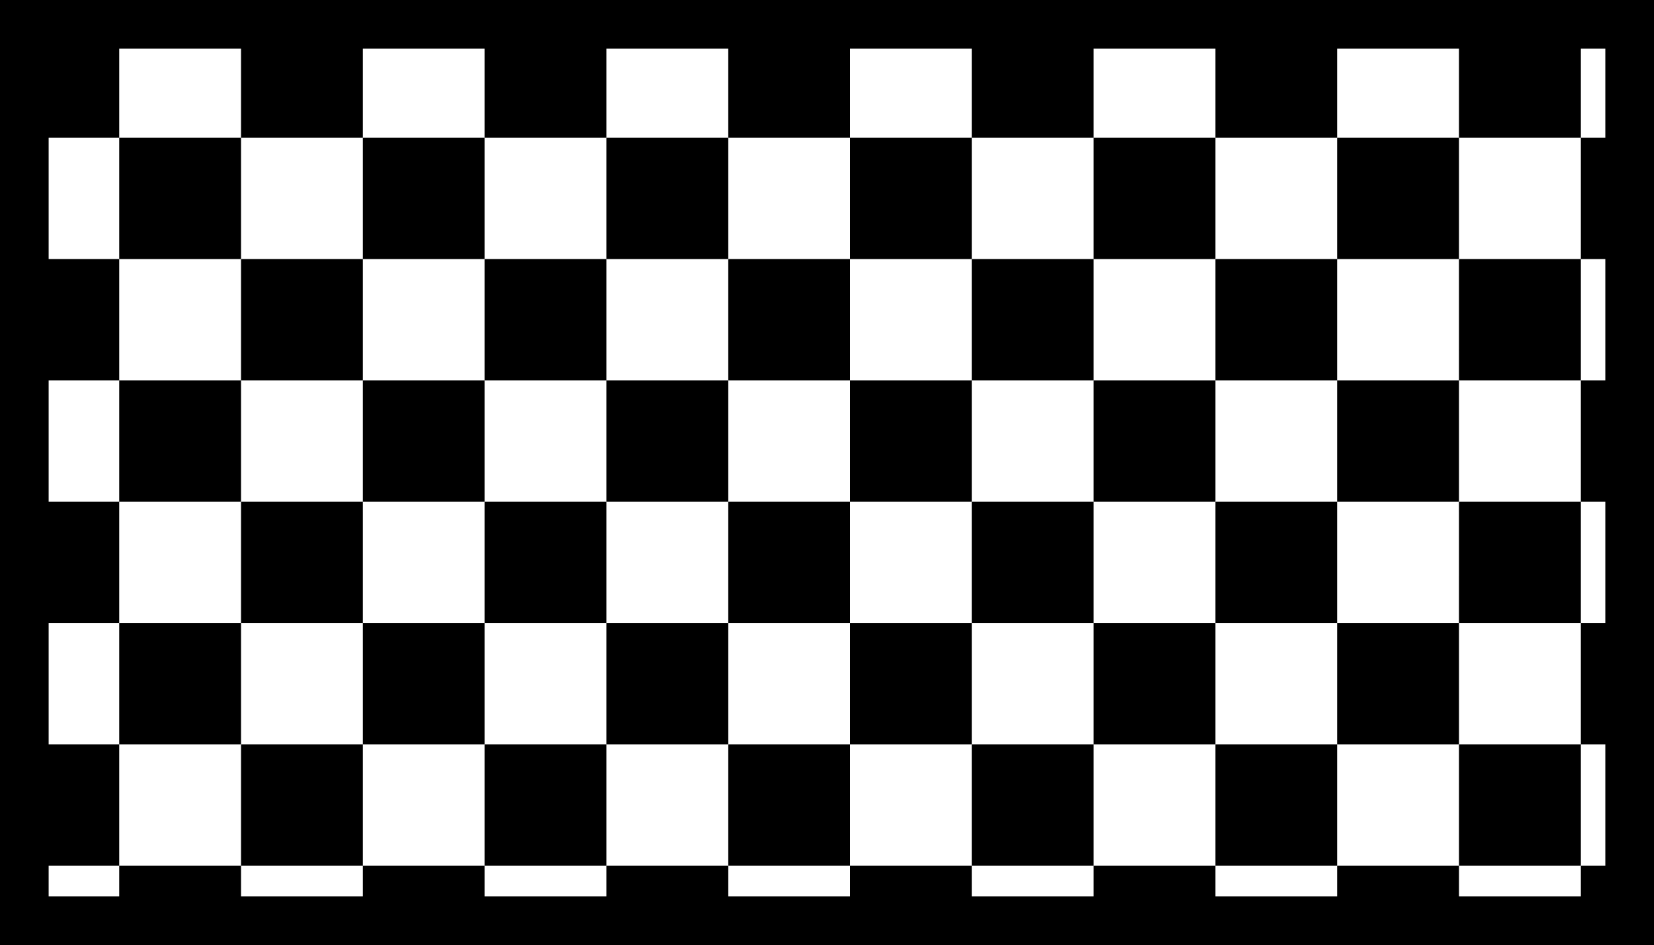
\includegraphics[width=.8\textwidth]{media/1600wind.png}
    \caption{Recovery dispersion with wind typical to 16:00 on the site.}
\end{figure}
\subsubsection{1-$\sigma$ RS-Pro Uncertainties}
\paragraph{Mass Properties}
\begin{table}[H]
    \centering
    \caption{RS-Pro mass property uncertainty}
    \begin{tabular}{|l|l|}
        \hline
        Mass & \ph\% \\ \hline
        Moments of Inertia & \ph \\ \hline
        Center of Gravity & \ph \\ \hline
    \end{tabular}
\end{table}
\paragraph{Aerodynamics}
\begin{table}[H]
    \centering
    \caption{RS-Pro aerodynamics uncertainty}
    \begin{tabular}{|l|l|}
        \hline
        $C_a$ & \ph \% \\ \hline
        $C_n$ & \ph \% \\ \hline
        CP & \ph cal \% \\ \hline
        Fin Cant & \ph$^\circ$ \\ \hline
    \end{tabular}
\end{table}
\paragraph{Propulsion}
\begin{table}[H]
    \centering
    \caption{Rs-Pro Propulsion uncertainty}
    \begin{tabular}{|l|l|}
        \hline
        Total Impulse & \ph \% \\ \hline
        Propellant & \ph \% \\ \hline
        Thrust Axis & \ph $^\circ$ \\ \hline
    \end{tabular}
\end{table}
\paragraph{Wind}
\begin{table}[H]
    \centering
    \caption{RS-Pro wind uncertainty}
    \begin{tabular}{|l|l|}
        \hline
        Direction & \ph $^\circ$ \\ \hline
        Velocity & \ph fps \\ \hline
    \end{tabular}
\end{table}
\paragraph{Launch Rail}
\begin{table}[H]
    \centering
    \caption{RS-Pro launch rail uncertainty}
    \begin{tabular}{|l|l|}
        \hline
        Azimuth & \ph $^\circ$ \\ \hline
        Elevation & \ph $^\circ$ \\ \hline
    \end{tabular}
\end{table}
\paragraph{Failure Likelihood}
\begin{table}[H]
    \centering
    \caption{RS-Pro failure likelihood factors.}
    \begin{tabular}{|l|l|}
        \hline
        Ignition & \ph \% \\ \hline
        C.A.T.O. & \ph \% \\ \hline
        Deployment & \ph \% \\ \hline
        Chute Failure & \ph \% \\ \hline
    \end{tabular}
\end{table}
\section{Supporting Systems}
\subsection{Radio Communication}
To facilitate prompt and resilient communication while on site and performing recovery operations,
10-watt 2-meter band HAM radios will be used.
All radios will be operated by persons licensed per 47 CFR 97.503(a).
All radios may be operated in a mode to comply with 47 CFR 95.531 through 47 CFR 95.587 for use on FRS channels.

The telemetry enabled systems onboard the rocket operate on the 70-centimeter HAM band.
These signals will be received by two offsite 5-element Yagi-Uda antennas with a gain of 6 dbi.
Each will be equipped with appropriate computer hardware to interpret the signals.
\section{Safety Procedures}
\begin{enumerate}[label=(\alph*)]
    \item Range safety, pre-, during- and post-launch checklists will be used.
    \item Event operators will be alerted to all actions.
    \item The team will communicate readiness to launch to the Launch Control Officer,
    who will provide setup instructions and decide the order of launches.
    \item The Launch Control Officer will alert event attendees via a public address system.
\end{enumerate}
\section{Mishap and Emergency Procedures \& Facilities}
\begin{enumerate}[label=(\alph*)]
    \item Basic first aid available on site.
    \item Nearest hospital located in \ph, \ph miles away.
    \item Nearest fire and rescue located in \ph, \ph miles away.
    \item Procedures and provisions for extinguishing fires initiated by motor ignition are present on site per agreement with the Forest Service.

\end{enumerate}
\end{document}